\chapter{Rules-Based Agent}

Rules-based AI agents in board games operate on predefined sets of rules and strategies programmed by developers. These agents analyze the game state, 
evaluate available moves, and select the best course of action based on a predetermined set of rules. 


My rules-based agents assess the potential moves within the current state but refrain from delving deeper into constructing a comprehensive tree of 
possible game states by exploring multiple move sequences across various depths. This implies that the rules-based agents don't have to deal with
imperfect information since all the information is available at the current state and they don't look beyond the current move.


\section{Only Die To Field Move Strategy}

As the name suggests, this strategy of the rules-based agent makes only moves that place a die onto a field i.e. it doesn't use any Tool Cards.
The main reason for having this strategy is connected to performance because Tool Card moves contribute significantly to the average branching factor.
Agents using this strategy not only don't have to consider using Tool Card moves but they save time by not even generating the Tool Card moves.

The rules-based agents don't use the heuristic filter and the heuristic sort functionalities. The algorithm begins
with saving information about the current state. After this, all the moves are tried out and the new states are compared with the initial one. The 
moves are evaluated using the following criteria:
\begin{enumerate}
    \item \textbf{Minimize the count of newly appearing fields that cannot be filled without using a relocating tool card} - Increasing the count of these fields potentially 
    leads to increasing uncompletable Public Objective Card patterns and empty fields at the end of the game. For this reason, if the algorithm encounters a move that increases
    this number compared to the current minimum, the move is immediately skipped.
    \item \textbf{Public Objective Card state} - I evaluate the state of the game from the perspective of the Public Objective Cards with a very similar heuristic function
    described in Section \ref{sec:Minimax_Heuristic_Function} .
    \item \textbf{Color of the die} - If the color of the die matches the color of the agent's Private Objective Card, the state value is increased by the weighted value
    of the die.
    \item \textbf{Total points achieved} - Finally, the total points achieved are compared to the current best move's total points.
\end{enumerate} 

The algorithm updates the current best move if the processed move shows better results in the Public Objective Card state and the Total points achieved components.


\section{All Moves Strategy}

The algorithm begins with separating all the possible moves into three categories: relocating tool card moves, tool card moves that contain randomness and all the other 
moves including die-placing moves and other tool card moves. First, the relocating moves are processed. The main criterion followed is to choose the move
that makes the number of uncompletable fields the minimum possible. If there is at least one such move, it will be used. Second, using the algorithm described
in the previous section, I evaluate the die-placing moves and all the tool card moves that contain placing a die onto a field as a sub-move. If die-placing move selected by the
Only Die To Field Move Strategy has a positive heuristic value, it will be chosen as the main move. Otherwise, if there are any moves
containing randomness, a random one of these moves will be chosen. Finally, if none of the previous actions led to a final move, the very first possible move will be chosen.

\section{Branching Factors}

To demonstrate the difference in performance, I ran 1000 games between two agents using the two different strategies. The following plot visualizes
the average branching factor over 1000 games:


\begin{figure}[H]
    \caption{ Branching factor across the rounds for the two rules-based strategies}
    \centerline{\mbox{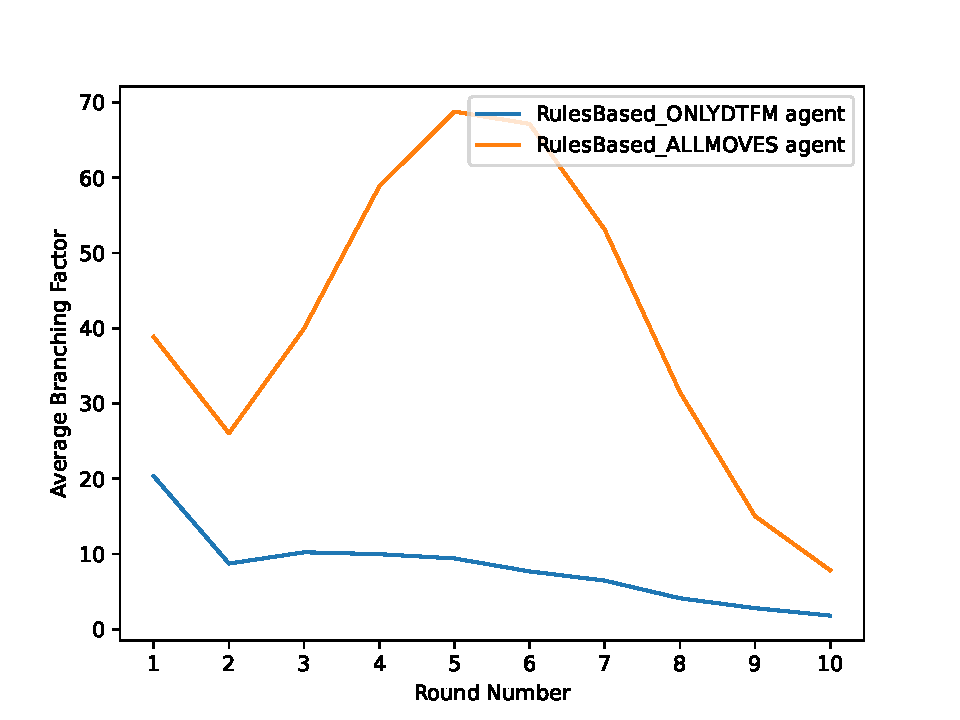
\includegraphics[width=150mm]{img/rules-based_agents_branching_factor.pdf}}}
    \label{fig:example}
\end{figure}
